\documentclass[prb,papersize=a4paper,notitlepage]{revtex4-1}%
\usepackage{hyperref}
\usepackage{enumitem}
\usepackage{nicefrac}
\usepackage{amsmath}
\usepackage{graphicx}
\usepackage{amsfonts}
\usepackage{physics}
\usepackage{amssymb}
\usepackage{bm}
\usepackage[utf8]{inputenc}
\usepackage[russian]{babel}
\usepackage{listings}


\begin{document}

\title{Вычислительная физика, Осень 2020 ВШЭ. Задание 3.\footnote{Дополнительно указаны: (количество баллов за задачу)[имя задачи на nbgrader]}}
\maketitle


\begin{enumerate}
\item \textbf{(7)} Покажите, что:
\begin{itemize}
\item проектор $P$ является ортогональным если и только если $P = P^T$
\item если $P$ -- ортогональный проектор, то матрица $I-2P$ унитарна (дайте геометрическую интерпретацию этого факта).
\end{itemize}

\item \textbf{(7)} Рассмотрите матрицы:
$$
A=\quad\begin{bmatrix}
1 & 0\\
0 & 1\\
1 & 0
\end{bmatrix},\quad
B=\quad\begin{bmatrix}
1 & 2\\
0 & 1\\
1 & 0
\end{bmatrix}.
$$
\begin{itemize}
\item Выпишите ортогональные проекторы на $\mathrm{range}(A)$ и $\mathrm{range}(B)$.
\item Постройте руками QR разложение матриц $A$ и $B$.
\end{itemize}

\item \textbf{(15)} Допишите следующий код на Python так, чтобы он генерировал матрицу $A$ (состоящую из 0 и 1) размера $15\times 28$, показанную на Рис. 1 (для визуализации матрицы использована функция \lstinline{plt.imshow(A)}):
\lstset{language=Python}
\lstset{frame=lines}
\lstset{label={lst:code_direct}}
\lstset{basicstyle=\ttfamily}
\begin{lstlisting}
a = np.zeros((15, 28))
a[2:-2,1] = 1; a[2,2:6] = 1
a[2:7,6] = 1; a[7:-2,7] = 1
a[7,2:7] = 1; a[-3,2:7] = 1
a[2:-2, 10] = 1; a[2:-2, 14] = 1; 
a[2:-2, 18] = 1; a[-3,10:19] = 1
\end{lstlisting}
\begin{figure}[h!]
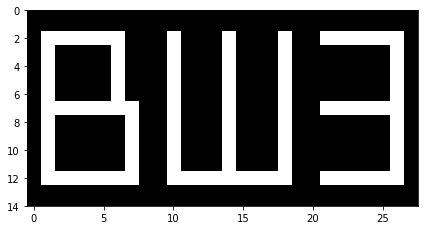
\includegraphics[width=8cm]{hse.png}
\caption{Матрица $A$, задача 3.}
\label{subs}
\end{figure}
\begin{itemize}
\item Постройте SVD разложение матрицы $A$. Чему равен $\mathrm{rank(A)}$?
\item Для каждого $i=1,2,...,\mathrm{rank}(A)$, постройте матрицу $B_i$ ранга $i$, которая наилучшим образом (в 2-норме) приближает матрицу $A$ (постройте соответствующее изображение). 
\end{itemize}

\item \textbf{(15)} Реализуйте \href{https://github.com/ev-br/CP2020/blob/master/week_3_lsq.ipynb}{метод наименьших квадратов}, следуя инструкциям по ссылке.

\item \textbf{(15)} 
Рассмотрите единичную массу, находящуюся при $t=0$ в точке $x=0$ в состоянии покоя $v=0$ и подверженную силе $f_i$ при $i-1< t \le i$, где $i=1,2,...,10$. Пусть $a=(x(t=10),v(t=10))$ -- вектор, состоящий из координаты и скорости частицы в момент времени $t=10$. Постройте матрицу $A$ такую, что $a=Af$ (заметьте, что $A$ имеет размер $2\times 10$). Используя SVD разложение, найдите $f$ минимальной нормы такое, что $a=(1,0)$.
\end{enumerate}
\end{document}